To set up the hardware, one can either:
\begin{itemize}
	\item Build the design himself as described in the previous sections
	\item Use the prebuilt files provided in \emph{<repo>/prebuilt}
\end{itemize}

Five partitions must be created and formatted on an SD card of at least $4GB$. These partitions contain the following files:
\begin{itemize}
    \item BOOT partition:
    \begin{itemize}
        \item BOOT.BIN: Contains the \gls{fsbl}, \gls{pmufw}, u-boot, ARM Trusted Firmware and the bitstream for the \gls{pl}
        \item Image: The linux kernel
        \item uramdisk.img: The ramdisk for Android
        \item zynqmp-zcu102-rev1.0.dtb: The compiled devicetree
        \item uEnv.txt: The kernel parameters 
    \end{itemize}
    
    \item CACHE partition:
    \begin{itemize}
        \item left empty
    \end{itemize}
    
    \item DATA partition:
    \begin{itemize}
        \item startup.sh: The script that loads the kernel modules
        \item modules/blake2b.ko: The kernel driver for the hasing device
        \item modules/blake2b.ko: The kernel driver for the image filters
        \item Root\_Client.sh: The script that forwards the commands from the app to the kernel drivers
    \end{itemize}
    
    \item ROOT partition:
    \begin{itemize}
        \item left empty
    \end{itemize}
    
    \item SYSTEM partition:
    \begin{itemize}
        \item system.img: Contains Android system files. This image is extracted to the partition. 
    \end{itemize}
\end{itemize}

To create this partition structure, the following command can be executed. All necessary files are also written to the respective partition.
\begin{lstlisting}[
	language=Bash,
	%caption={Preparing SD Card},
	%label={lst:preparesd},
	basicstyle=\small,
	float=htbp,
	floatplacement=htbp
	]
# Use the path to your SD card instead of '/dev/mmcblk0'
sudo bootimage/mkSDcard.sh /dev/mmcblk0 populate
\end{lstlisting}
\FloatBarrier

Follow the steps below to set up the ZCU102:
\begin{itemize}
    \item Use ZCU102 User Guide \cite{UG1182} as a reference for switches and connectors location
    \item Set boot mode of the board to "SD Boot"
    \item Insert SD card to the board
    \item Connect external monitor using DisplayPort. Please note that DP must be connected before board power-on
    \item Connect USB mouse, USB keyboard and the USB touchscreen connector using an USB hub
    \item An Ethernet cable can be connected to the Ethernet port
    \item A \gls{uart} interface is available at the \gls{uart} USB port.
\end{itemize}

The setup can be seen in \cref{fig:zcu102setup}.

\begin{figure}[htbp]
    \centering
    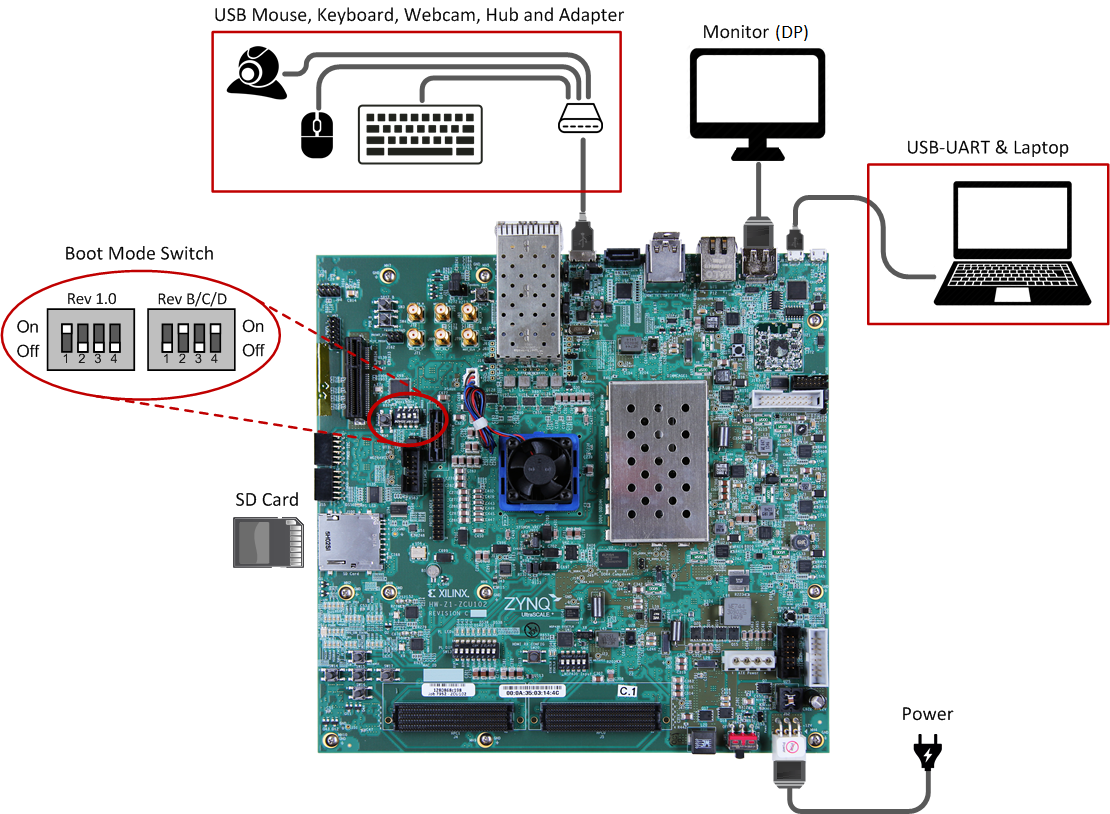
\includegraphics[width=1\textwidth]{images/ZCU102.png}
    \caption{\label{fig:zcu102setup} ZCU102 setup}
\end{figure}

Once everything is set up, the power switch can be switched to the \emph{ON}
position and Android will boot.
After boot, Android will present itself on the display and show the launcher
as seen in \Cref{fig:androiddisplay}.

\emph{NOTE:} The screen must be connected before boot, otherwise the Android
\gls{gui} will not show.

\begin{figure}[htbp]
    \centering
    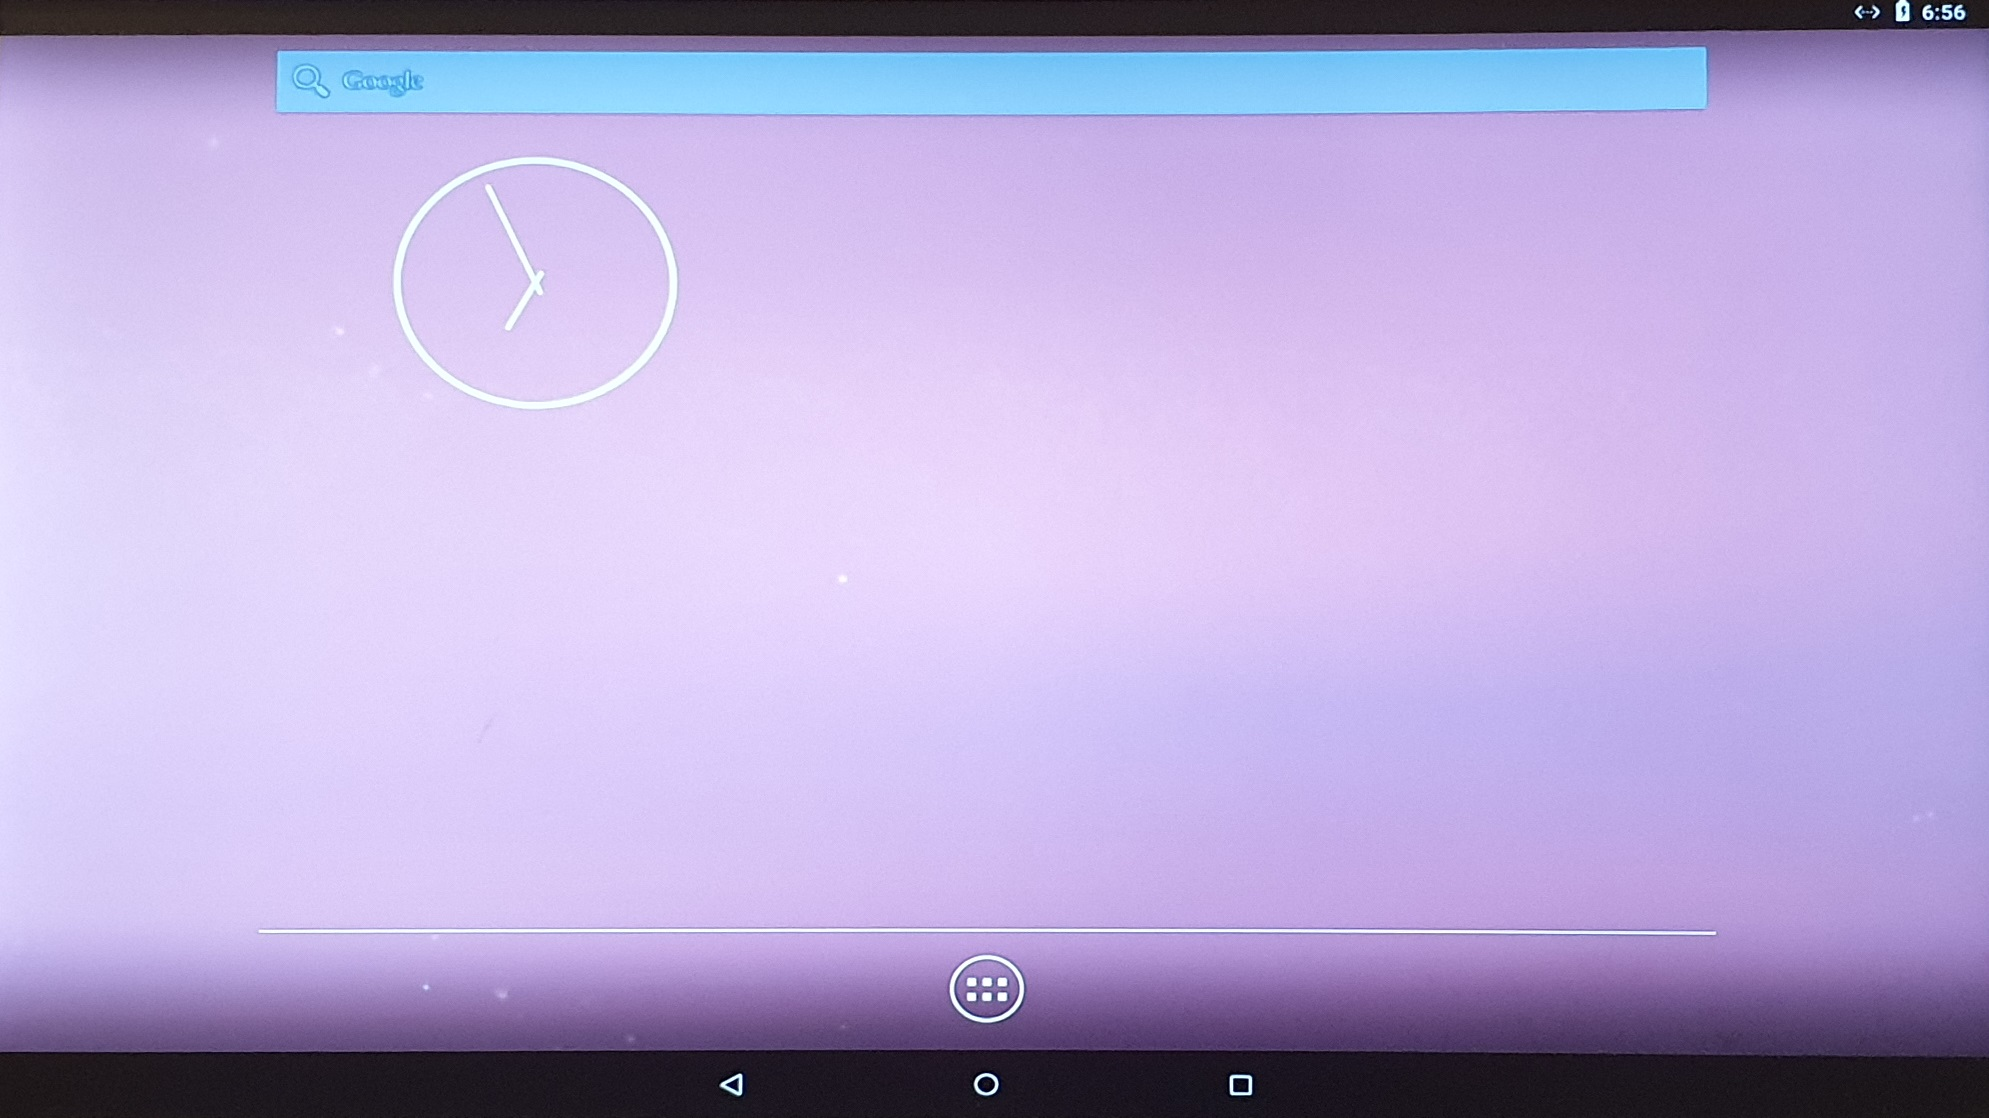
\includegraphics[width=1\textwidth]{images/android-launcher.jpg}
    \caption{\label{fig:androiddisplay} Android 8 launcher}
\end{figure}
